
\chapter{Introduction}
\label{chap:introduction}

Recovering visual information from brain activity is one of the most ambitious goals of modern computational neuroscience. In recent years, large-scale neuroimaging datasets, multimodal representation learning, and generative models have enabled a shift from coarse category decoding toward image-specific retrieval and plausible visual reconstruction from fMRI signals \cite{Allen2022,Ozcelik2023,Scotti2023,Scotti2024}. This progress is scientifically important because it connects two difficult problems: understanding how the visual cortex represents semantic and structural information, and learning machine representations that can act as bridges between biological measurements and natural images.

The present thesis focuses on the \emph{visual perception} setting. During each trial, a subject observes a natural image and the corresponding blood-oxygen-level-dependent (BOLD) response is recorded with high-field fMRI. The central task is to infer an image-aligned latent representation from this neural signal. Rather than predicting pixels directly, the pipeline maps fMRI activity into a CLIP-based embedding space, where similarity can be measured reliably and where downstream diffusion-based image generation becomes possible \cite{Radford2021,Rombach2022}. This choice turns the problem into a structured latent prediction task rather than a fragile direct image regression problem.

Formally, let $x_i \in \mathbb{R}^{V}$ denote the preprocessed voxel vector for trial $i$, where $V$ is the number of selected voxels, and let $z_i \in \mathbb{R}^{d}$ denote the target image embedding extracted from a pretrained vision-language model. The decoder is a parametric mapping
\begin{equation}
\hat{z}_i = f_{\theta}(x_i), \qquad f_{\theta}: \mathbb{R}^{V} \rightarrow \mathbb{R}^{d},
\label{eq:intro_mapping}
\end{equation}
where $\hat{z}_i$ should preserve enough image-specific information to retrieve the correct image from a held-out gallery and, later, to condition a generative model. The main evaluation scenario is therefore retrieval: for each predicted embedding, the system searches a gallery of candidate images and ideally ranks the ground-truth item first.

This formulation is challenging for several reasons. First, fMRI is an indirect and noisy measurement of neural activity, with low temporal resolution and substantial inter-session variability \cite{Allen2022,Wen2018}. Second, the representation space of modern visual models is high-dimensional and geometrically nontrivial \cite{Radford2021,Conneau2018}. Third, there is a constant risk of data leakage or protocol mismatch when repeated images, subject-specific preprocessing, and cached features are involved. A strong bachelor thesis in this area must therefore be both algorithmically ambitious and experimentally rigorous.

The main research question of this thesis is the following: \emph{how can one learn a stable mapping from cortical activity to an image-aligned latent space that supports accurate retrieval and provides a credible foundation for visual reconstruction?} The project approaches this question through an iterative experimental program. Early stages establish robust baselines and eliminate implementation errors. Later stages explore probabilistic decoders, directional losses, richer targets, multi-head retrieval designs, and shortlist-based fusion strategies.

\section{Motivation and Context}

The work is motivated by the convergence of three research directions. The first is the availability of datasets such as the Natural Scenes Dataset, which provide image-level behavioural and neuroimaging data at a scale that was previously unavailable \cite{Allen2022}. The second is the emergence of CLIP-style multimodal latent spaces, which align image representations with semantic structure and perform well in retrieval settings \cite{Radford2021}. The third is the success of latent diffusion models, which make it possible to turn recovered latent information into realistic image samples \cite{Rombach2022,Ozcelik2023,Takagi2023}. Together, these directions make fMRI-to-image decoding both more realistic and more measurable than in earlier generations of brain-decoding systems.

\begin{figure}[htbp]
    \centering
    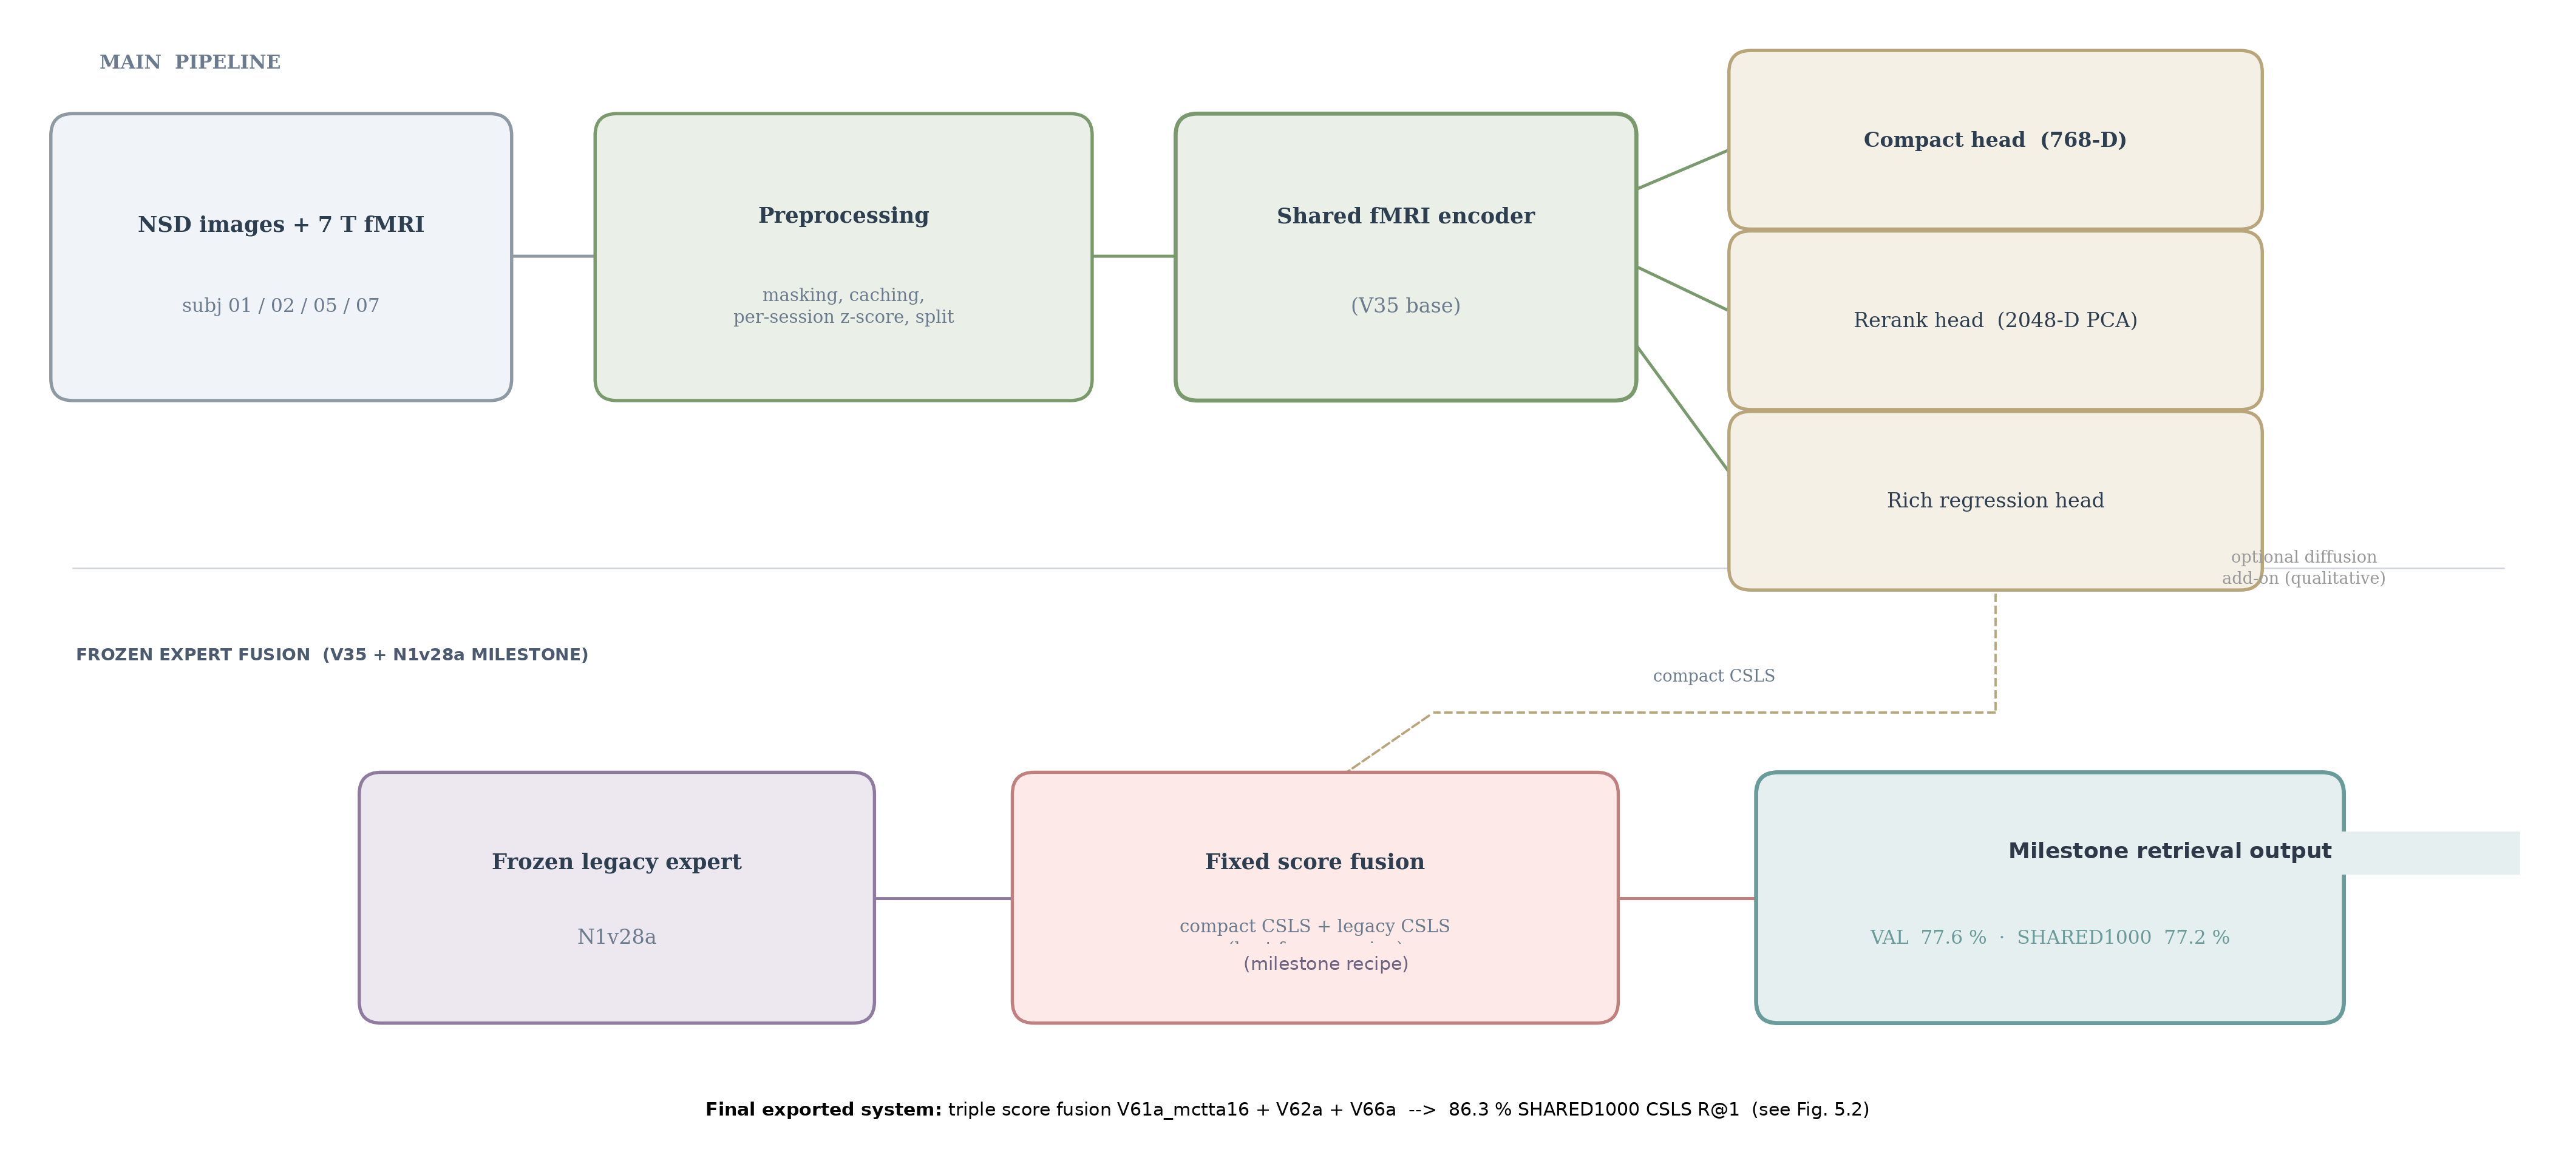
\includegraphics[width=\textwidth]{thesis_pipeline.png}
    \caption{Overview of the complete thesis pipeline. The written thesis is centered on retrieval: NSD fMRI is preprocessed and mapped by a shared encoder into compact, rerank, and rich latent heads. The V35 plus frozen legacy N1v28a fixed fusion is retained as a methodological milestone, while the final exported system is a frozen cross-architecture triple score fusion that combines a 197K token-space model with MC-TTA, a 768-D CLS model, and a 768-D ROI-pretrained model. The diffusion add-on is treated as an optional qualitative extension rather than as the primary benchmark.}
    \label{fig:thesis_pipeline}
\end{figure}

A complementary single-example view is useful because it makes the retrieval-first logic concrete. Starting from one viewed stimulus and its matched cortical response, the thesis builds a CLIP target embedding from the image, learns a brain-to-latent mapping from the associated fMRI activity, and then evaluates the predicted latent first through held-out retrieval and only secondarily through optional qualitative generation.

\begin{figure}[htbp]
    \centering
    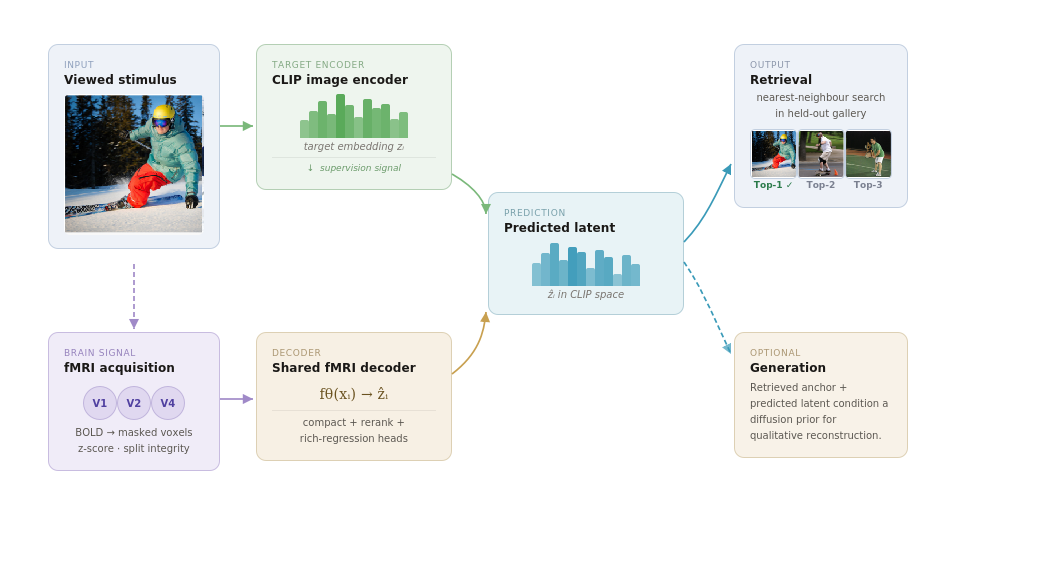
\includegraphics[width=0.94\textwidth]{end_to_end_example_pipeline.png}
    \caption{Single-example decoding path used throughout the thesis. A viewed image defines the target CLIP embedding, the corresponding fMRI response is preprocessed into a voxel vector, and the decoder learns to map that brain activity into the shared latent space used for retrieval-first evaluation and optional downstream generation.}
    \label{fig:end_to_end_example_pipeline}
\end{figure}

\section{Objectives of the Thesis}

The thesis has four concrete objectives:
\begin{itemize}
    \item to construct a reproducible pipeline for mapping fMRI activity to CLIP-aligned visual embeddings;
    \item to evaluate how architectural and loss-design choices affect retrieval quality under a leakage-free protocol;
    \item to analyse why some experimentally attractive ideas fail, especially under hubness and representation-geometry constraints;
    \item to validate a multi-stage retrieval strategy in which compact retrieval, dedicated reranking, and frozen score-level fusion across complementary experts are treated as distinct but cooperative inference mechanisms.
\end{itemize}

These objectives are intentionally both scientific and engineering-oriented. The final artifact is not only a set of metric values, but also a structured experimental framework in which preprocessing, target caching, training, evaluation, qualitative analysis, and implementation validation are integrated into a single research pipeline.

\section{Original Contributions of the Author}

The original contributions emphasized in this thesis are the following:
\begin{itemize}
    \item the design and implementation of an end-to-end fMRI-to-latent decoding pipeline built around NSD, CLIP targets, and retrieval-based evaluation;
    \item a systematic debugging and validation program addressing alignment, split integrity, checkpoint selection, and retrieval geometry;
    \item an experimental comparison between single-head, dual-head, and triple-head retrieval formulations under a shared protocol;
    \item the validation of shortlist-local reranking as a corrective mechanism, followed by a stronger frozen fixed-fusion milestone built on the V35 compact expert and the legacy N1v28a expert, and finally extended into a frozen cross-architecture triple score fusion that combines a 197K token-space model with MC-TTA and two complementary 768-D experts as the final exported retrieval system;
    \item a conservative qualitative analysis of retrieval-guided diffusion refinement, showing where anchor-preserving generation is useful and where exact retrieval should remain unchanged;
    \item the explicit documentation of negative results and failed directions, which is scientifically useful because it narrows future search space.
\end{itemize}

At the time of writing, the work has not yet been presented as a peer-reviewed conference publication. The thesis therefore serves as the primary written record of the experimental results, methodological design, and implementation choices.

\section{Transparency Regarding the Use of Generative AI Tools}

In accordance with the university guidelines, the author states transparently that generative AI tools were used only in a limited and assistive manner during the preparation of the manuscript. Their use was restricted to language polishing, reformulation suggestions, and LaTeX refactoring support. The scientific content, literature verification, experimental design, software implementation, numerical results, and interpretation of findings remain the full responsibility of the author. No generative AI system is treated as an author or as an authoritative source of scientific truth.

\section{Structure of the Thesis}

The remainder of the thesis is organized as follows. Chapter~\ref{chap:background} reviews the theoretical background, the relevant literature, the historical evolution of the field, the NSD dataset, and the main evaluation metrics used in the project. Chapter~\ref{chap:methodology} presents the proposed methodology, including preprocessing, target construction, model design, and the multi-head retrieval formulation. Chapter~\ref{chap:implementation} describes the software design, experiment management, validation strategy, and reproducibility measures of the implemented system. Chapter~\ref{chap:experiments} reports the experimental evolution of the project, summarizes the main results, and discusses their scientific interpretation. Finally, Chapter~\ref{chap:conclusions} summarizes the conclusions, limitations, and future directions.
